
\section{Test Deployment}\label{app:test-deployment}

Figure~\ref{fig:test-deployment} shows the architecture diagram of the deployment that was used to test this application. Some notes about it are:

\begin{itemize}
  \item The smart contract code is deployed to the Sepolia test-net.
  \item I am interfacing with Sepolia using a node being run by Alchemy. Alchemy provide an RPC URL that we use in the application to connnect to Sepolia.
  \item I am using the Kubo implementation of IPFS that is connected to via a daemon process being run locally.
\end{itemize}

\begin{figure}[ht]
  \centering
  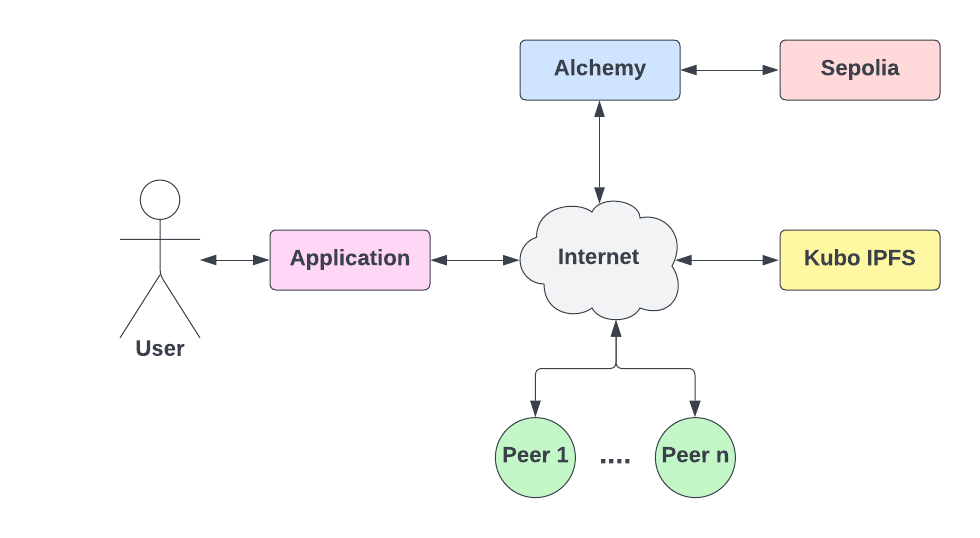
\includegraphics[width=.9\textwidth]{assets/images/diagrams/test-deployment.png}
  \caption{The architecture of the deployment used for testing.}
  \label{fig:test-deployment}
\end{figure}